\documentclass[a4paper,12pt,3p]{report}

\usepackage{graphicx}
\usepackage[font=normalsize]{caption}
\usepackage{subcaption}
\usepackage{float}
\usepackage{wrapfig}
\usepackage{amssymb}
\usepackage{amsmath}
\usepackage{amstext}
\usepackage[linesnumbered,ruled]{algorithm2e}
\usepackage{multicol}
\usepackage{multirow}


\usepackage[bookmarks=false]{hyperref}
\hypersetup{colorlinks,
	linkcolor=blue,
	citecolor=blue,
	urlcolor=blue}
\usepackage{titlesec}
\setcounter{secnumdepth}{4}

%\usepackage{csquotes}
%\usepackage[style=verbose-ibid,backend=bibtex]{biblatex}
%\bibliography{reference}

\titleformat{\paragraph}
{\normalfont\normalsize\bfseries}{\theparagraph}{0.5em}{}
\titlespacing*{\paragraph}
{0pt}{1.25ex plus 1ex minus .2ex}{0.5ex plus .2ex}
\graphicspath{ {./images/} }
\usepackage[X2,T1]{fontenc}
\usepackage[utf8]{vietnam}
\usepackage{tabu}

\DeclareTextSymbolDefault{\CYREPS}{X2}
\DeclareTextSymbolDefault{\cyreps}{X2}

\DeclareUnicodeCharacter{0190}{\CYREPS}
\DeclareUnicodeCharacter{025B}{\cyreps}
\usepackage[left=2cm,right=2cm,top=2cm,bottom=3cm]{geometry}
\usepackage{indentfirst}
\usepackage{color, colortbl}
\definecolor{Gray}{gray}{0.9}

\usepackage{graphicx}
\graphicspath{{./images/}}	% declare the path(s) where your graphic files are
\DeclareGraphicsExtensions{.pdf,.jpeg,.png} % and their extensions so you won't have to specify these with every instance of \includegraphics
%%%%%%%%%%%%%%%%%%%%%%%%%%%%%%%%%%%%%%%%%%%%%%%%%%%%%%%%%%%%%%%%%%%%%%%%%%%%%%%%%%%%%%%%%%%

\usepackage{graphicx}
\usepackage{verbatim}
\usepackage{latexsym}
\usepackage{mathchars}
\usepackage{setspace}
\usepackage{footnote}

\setlength{\parskip}{\medskipamount}  % a little space before a \par
\setlength{\parindent}{0pt}	      % don't indent first lines of paragraphs
%UHEAD.STY  If this is included after \documentstyle{report}, it adds
% an underlined heading style to the LaTeX report style.
% \pagestyle{uheadings} will put underlined headings at the top
% of each page. The right page headings are the Chapter titles and
% the left page titles are supplied by \def\lefthead{text}.

% Ted Shapin, Dec. 17, 1986

\makeatletter
\def\chapapp2{Chapter}

\def\appendix{\par
 \setcounter{chapter}{0}
 \setcounter{section}{0}
 \def\chapapp2{Appendix}
 \def\@chapapp{Appendix}
 \def\thechapter{\Alph{chapter}}}

\def\ps@uheadings{\let\@mkboth\markboth
% modifications
\def\@oddhead{\protect\underline{\protect\makebox[\textwidth][l]
		{\sl\rightmark\hfill\rm\thepage}}}
\def\@oddfoot{}
\def\@evenfoot{}
\def\@evenhead{\protect\underline{\protect\makebox[\textwidth][l]
		{\rm\thepage\hfill\sl\leftmark}}}
% end of modifications
\def\chaptermark##1{\markboth {\ifnum \c@secnumdepth >\m@ne
 \chapapp2\ \thechapter. \ \fi ##1}{}}%
\def\sectionmark##1{\markright {\ifnum \c@secnumdepth >\z@
   \thesection. \ \fi ##1}}}
\makeatother
%%From: marcel@cs.caltech.edu (Marcel van der Goot)
%%Newsgroups: comp.text.tex
%%Subject: illegal modification of boxit.sty
%%Date: 28 Feb 92 01:10:02 GMT
%%Organization: California Institute of Technology (CS dept)
%%Nntp-Posting-Host: andromeda.cs.caltech.edu
%%
%%
%%Quite some time ago I posted a file boxit.sty; maybe it made it
%%to some archives, although I don't recall submitting it. It defines
%%	\begin{boxit}
%%	...
%%	\end{boxit}
%%to draw a box around `...', where the `...' can contain other
%%environments (e.g., a verbatim environment). Unfortunately, it had
%%a problem: it did not work if you used it in paragraph mode, i.e., it
%%only worked if there was an empty line in front of \begin{boxit}.
%%Luckily, that is easily corrected.
%%
%%HOWEVER, apparently someone noticed the problem, tried to correct it,
%%and then distributed this modified version. That would be fine with me,
%%except that:
%%1. There was no note in the file about this modification, it only has my
%%   name in it.
%%2. The modification is wrong: now it only works if there is *no* empty
%%   line in front of \begin{boxit}. In my opinion this bug is worse than
%%   the original one.
%%
%%In particular, the author of this modification tried to force an empty
%%line by inserting a `\\' in the definition of \Beginboxit. If you have
%%a version of boxit.sty with a `\\', please delete it. If you have my
%%old version of boxit.sty, please also delete it. Below is an improved
%%version.
%%
%%Thanks to Joe Armstrong for drawing my attention to the bug and to the
%%illegal version.
%%
%%                                          Marcel van der Goot
%% .---------------------------------------------------------------
%% | Blauw de viooltjes,                    marcel@cs.caltech.edu
%% |    Rood zijn de rozen;
%% | Een rijm kan gezet
%% |    Met plaksel en dozen.
%% |


% boxit.sty
% version: 27 Feb 1992
%
% Defines a boxit environment, which draws lines around its contents.
% Usage:
%   \begin{boxit}
%	... (text you want to be boxed, can contain other environments)
%   \end{boxit}
%
% The width of the box is the width of the contents.
% The boxit* environment behaves the same, except that the box will be
% at least as wide as a normal paragraph.
%
% The reason for writing it this way (rather than with the \boxit#1 macro
% from the TeXbook), is that now you can box verbatim text, as in
%   \begin{boxit}
%   \begin{verbatim}
%   this better come out in boxed verbatim mode ...
%   \end{verbatim}
%   \end{boxit}
%
%						Marcel van der Goot
%						marcel@cs.caltech.edu
%

\def\Beginboxit
   {\par
    \vbox\bgroup
	   \hrule
	   \hbox\bgroup
		  \vrule \kern1.2pt %
		  \vbox\bgroup\kern1.2pt
   }

\def\Endboxit{%
			      \kern1.2pt
		       \egroup
		  \kern1.2pt\vrule
		\egroup
	   \hrule
	 \egroup
   }	

\newenvironment{boxit}{\Beginboxit}{\Endboxit}
\newenvironment{boxit*}{\Beginboxit\hbox to\hsize{}}{\Endboxit}
\pagestyle{empty}

\setlength{\parskip}{2ex plus 0.5ex minus 0.2ex}
\setlength{\parindent}{0pt}

\makeatletter  %to avoid error messages generated by "\@". Makes Latex treat "@" like a letter

\linespread{1.5}
\def\zzfl@error{Float(s) lost}
\def\submitdate#1{\gdef\@submitdate{#1}}
\def\maketitle{
  \begin{titlepage}{
    %\linespread{1.5}
    \Large HANOI UNIVERSITY OF SCIENCE AND TECHNOLOGY \\
    %\linebreak
    School of Information and Comunication Technology \\
    %\linebreak
    *****
    \rm
    \vskip 0.5in
    
\includegraphics[width=0.2 \textwidth]{images/hust} 
    \vskip 0.5in
    \Large \bf GRADUATION THESIS\par
    \Large \flushleft Topic:\par
    \Large \center \bf \@title \par
  }

  \vskip 0.3in
  \par
 % \begin{flushright}
  {\Large Author: \bf \@author} 
  \vskip 0.1in
  \Large Supervisor: \bf PhD. Binh Minh Nguyen
%	\end{flushright}
  \par
  \vskip 2in
  \par
  
  \@submitdate
  \vfil
  \end{titlepage}
}

\def\titlepage{
  \newpage
  \centering
  \linespread{1}
  \normalsize
  \vbox to \vsize\bgroup\vbox to 9in\bgroup
}
\def\endtitlepage{
  \par
  \kern 0pt
  \egroup
  \vss
  \egroup
  \cleardoublepage
}

\def\abstract{
  \begin{center}{
    \Large\bf Tóm tắt}
  \end{center}
  \small
  %\def\baselinestretch{1.5}
  \linespread{1.5}
  \normalsize
}
\def\endabstract{
  \par
}

\newenvironment{sameauthor}{
	\cleardoublepage
	\begin{center}{
			\large \bf PHỤ LỤC 1: GIẤY XÁC NHẬN ĐỒNG TÁC GIẢ}
	\end{center}
	\small
	\linespread{1.5}
	\normalsize
}{\cleardoublepage}
\def\endsameauthor{
	\par
}


\newenvironment{acknowledgements}{
  \cleardoublepage
  \begin{center}{
    \large \bf Lời cảm ơn}
  \end{center}
  \small
  \linespread{1.5}
  \normalsize
}{\cleardoublepage}
\def\endacknowledgements{
  \par
}

\newenvironment{dedication}{
  \cleardoublepage
  \begin{center}{
    \large \bf Lời cam đoan}
  \end{center}
  \small
  \linespread{1.5}
  \normalsize
}{\cleardoublepage}
\def\enddedication{
  \par
}

\def\preface{

    \pagestyle{plain}
    \doublespacing
}

\def\body{
    \cleardoublepage    
    \pagestyle{uheadings}
    \tableofcontents
    \pagestyle{plain}
    \cleardoublepage
    \pagestyle{uheadings}
    \listoftables
    \pagestyle{plain}
    \cleardoublepage
    \pagestyle{uheadings}
    \listoffigures
    \pagestyle{plain}
    \cleardoublepage
    \pagestyle{uheadings}
    
    \doublespacing
}

\pagenumbering{arabic}
\makeatother  %to avoid error messages generated by "\@". Makes Latex treat "@" like a letter

\newcommand{\ipc}{{\sf ipc}}

\newcommand{\Prob}{\bbbp}
\newcommand{\Real}{\bbbr}
\newcommand{\real}{\Real}
\newcommand{\Int}{\bbbz}
\newcommand{\Nat}{\bbbn}

\newcommand{\NN}{{\sf I\kern-0.14emN}}   % Natural numbers
\newcommand{\ZZ}{{\sf Z\kern-0.45emZ}}   % Integers
\newcommand{\QQQ}{{\sf C\kern-0.48emQ}}   % Rational numbers
\newcommand{\RR}{{\sf I\kern-0.14emR}}   % Real numbers
\newcommand{\KK}{{\cal K}}
\newcommand{\OO}{{\cal O}}
\newcommand{\AAA}{{\bf A}}
\newcommand{\HH}{{\bf H}}
\newcommand{\II}{{\bf I}}
\newcommand{\LL}{{\bf L}}
\newcommand{\PP}{{\bf P}}
\newcommand{\PPprime}{{\bf P'}}
\newcommand{\QQ}{{\bf Q}}
\newcommand{\UU}{{\bf U}}
\newcommand{\UUprime}{{\bf U'}}
\newcommand{\zzero}{{\bf 0}}
\newcommand{\ppi}{\mbox{\boldmath $\pi$}}
\newcommand{\aalph}{\mbox{\boldmath $\alpha$}}
\newcommand{\bb}{{\bf b}}
\newcommand{\ee}{{\bf e}}
\newcommand{\mmu}{\mbox{\boldmath $\mu$}}
\newcommand{\vv}{{\bf v}}
\newcommand{\xx}{{\bf x}}
\newcommand{\yy}{{\bf y}}
\newcommand{\zz}{{\bf z}}
\newcommand{\oomeg}{\mbox{\boldmath $\omega$}}
\newcommand{\res}{{\bf res}}
\newcommand{\cchi}{{\mbox{\raisebox{.4ex}{$\chi$}}}}
%\newcommand{\cchi}{{\cal X}}
%\newcommand{\cchi}{\mbox{\Large $\chi$}}

% Logical operators and symbols
\newcommand{\imply}{\Rightarrow}
\newcommand{\bimply}{\Leftrightarrow}
\newcommand{\union}{\cup}
\newcommand{\intersect}{\cap}
\newcommand{\boolor}{\vee}
\newcommand{\booland}{\wedge}
\newcommand{\boolimply}{\imply}
\newcommand{\boolbimply}{\bimply}
\newcommand{\boolnot}{\neg}
\newcommand{\boolsat}{\!\models}
\newcommand{\boolnsat}{\!\not\models}


\newcommand{\op}[1]{\mathrm{#1}}
\newcommand{\s}[1]{\ensuremath{\mathcal #1}}

% Properly styled differentiation and integration operators
\newcommand{\diff}[1]{\mathrm{\frac{d}{d\mathit{#1}}}}
\newcommand{\diffII}[1]{\mathrm{\frac{d^2}{d\mathit{#1}^2}}}
\newcommand{\intg}[4]{\int_{#3}^{#4} #1 \, \mathrm{d}#2}
\newcommand{\intgd}[4]{\int\!\!\!\!\int_{#4} #1 \, \mathrm{d}#2 \, \mathrm{d}#3}

% Large () brackets on different lines of an eqnarray environment
\newcommand{\Leftbrace}[1]{\left(\raisebox{0mm}[#1][#1]{}\right.}
\newcommand{\Rightbrace}[1]{\left.\raisebox{0mm}[#1][#1]{}\right)}

% Funky symobols for footnotes
\newcommand{\symbolfootnote}{\renewcommand{\thefootnote}{\fnsymbol{footnote}}}
% now add \symbolfootnote to the beginning of the document...

\newcommand{\normallinespacing}{\renewcommand{\baselinestretch}{1.5} \normalsize}
\newcommand{\mediumlinespacing}{\renewcommand{\baselinestretch}{1.2} \normalsize}
\newcommand{\narrowlinespacing}{\renewcommand{\baselinestretch}{1.0} \normalsize}
\newcommand{\bump}{\noalign{\vspace*{\doublerulesep}}}
\newcommand{\cell}{\multicolumn{1}{}{}}
\newcommand{\spann}{\mbox{span}}
\newcommand{\diagg}{\mbox{diag}}
\newcommand{\modd}{\mbox{mod}}
\newcommand{\minn}{\mbox{min}}
\newcommand{\andd}{\mbox{and}}
\newcommand{\forr}{\mbox{for}}
\newcommand{\EE}{\mbox{E}}

\newcommand{\deff}{\stackrel{\mathrm{def}}{=}}
\newcommand{\syncc}{~\stackrel{\textstyle \rhd\kern-0.57em\lhd}{\scriptstyle L}~}

\def\coop{\mbox{\large $\rhd\!\!\!\lhd$}}
\newcommand{\sync}[1]{\raisebox{-1.0ex}{$\;\stackrel{\coop}{\scriptscriptstyle
#1}\,$}}

\newtheorem{definition}{Definition}[chapter]
\newtheorem{theorem}{Theorem}[chapter]

\newcommand{\Figref}[1]{Figure~\ref{#1}}
\newcommand{\fig}[3]{
 \begin{figure}[!ht]
 \begin{center}
 \scalebox{#3}{\includegraphics{figs/#1.ps}}
 \vspace{-0.1in}
 \caption[ ]{\label{#1} #2}
 \end{center}
 \end{figure}
}

\newcommand{\figtwo}[8]{
 \begin{figure}
 \parbox[b]{#4 \textwidth}{
 \begin{center}
 \scalebox{#3}{\includegraphics{figs/#1.ps}}
 \vspace{-0.1in}
 \caption{\label{#1}#2}
 \end{center}
 }
 \hfill
 \parbox[b]{#8 \textwidth}{
 \begin{center}
 \scalebox{#7}{\includegraphics{figs/#5.ps}}
 \vspace{-0.1in}
 \caption{\label{#5}#6}
 \end{center}
 }
 \end{figure}
}


\setlength{\parindent}{50pt}


\renewcommand{\baselinestretch}{2.0}
\DeclareUnicodeCharacter{2212}{-}
\begin{document}

\setlength{\abovedisplayskip}{3pt}
\setlength{\belowdisplayskip}{3pt}

\title{\LARGE {\bf Mô hình dự đoán chuỗi thời gian mờ đa chiều sử dụng LSTM và kĩ thuật phân tích\\ tương quan giữa các chiều dữ liệu \\áp dụng cho tài nguyên đám mây}\\
}

\author{Tran Quang Trung}
\submitdate{Hanoi, 12/2019}

\normallinespacing
\maketitle


\body
% body of thesis comes here

\chapter{Introduction}
\section{Problems}
\section{Summary}


\chapter{Materials and background}

\label{ch:background}

\section{Cloud Computing}
\section{Auto-scaling problem}
\section{Well-known machine learning models for Auto-scaling in cloud computing}
\label{ml_timeseries}

	Recent developments in cloud computing including resource management have resulted in a significant interest in resource usage prediction . Various methods have been proposed for solving this problem with different aspects, objectives and applications ~\cite{amiri2017survey}. In this section, we focus on several Artificial Neural Network (ANN) models that are used for tackling the time-series characteristic in resource usage forecast in cloud computing environment.
	Deep Feed-forward Neural Network, also called Feed-forward Neural Network (FFNN) are the quintessential deep learning models. The goal of all FFNN is to approximate some functions $f^*$.  In Regression problems, $y = f^*(x)$ maps an input $x$ to a value $y$. A feed-forward network defines a mapping $y = f(x,\theta)$ and learns the value of the parameters $\theta$ that result in the best function approximation. ~\cite{Goodfellow-et-al-2016}. These models are called feed-forward because information flows through the function being evaluated from $x$, through the intermediate computations used to define $f$, and finally to the output $y$. There are no feedback connections in which outputs of the model are fed back into itself. When feed-forward neural networks are extended to include feedback connections, they are called recurrent neural networks, which will be discussed in ~\ref{model_rnn}.
	
	In general, Multi-Layer Perceptrons (MLPs) models contain several disparate layers. The first layer is input layer taking information $x$ as input for the network. The last layer is called output layer, whose value is the result of $y$ with input $x$. The layers between the input and output layers are hidden layers. The structures of hidden layers are extremely diverse, varying from model to model. As presented in Fig. ***, a hidden layer of a simple FFNN is a group of neurons with no connection to each other, while in Recurrent Neural Networks (RNN), and Convolution Neural Network (CNN) hidden layer is a recurrent layer, and convolution layer respectively. 
	
	The Deep Neural Networks that are applied for Time series prediction will have input neurons presenting the historical data. The models utilize information from data in the past for forecasting future data. Input data presented as $x_1, x_2, ..., x_t$ is considered as historical values up to time t, which is used to predict the value at the time $t+1$. In other words, Deep Neural Networks will learn from data and approximate a function transforming the historical data up to time $t$ to the data at the time $t+1$ as follows:
\begin{equation} \label{eq_ffnn_1}
x(t+1) = y = f(x_1, x_2, ..., x_t)
\end{equation}
	
	 In this section, we summarize several Deep Neural Network models, which are widely used for time series forecasting. They are simple Multi-Layer Perceptrons (MLPs), Cascade Forward Neural Network (CFNN) and Recurrent-based Neural Network including traditional Recurrent Neural Network (RNN), Long-Short Term Memory (LSTM) and Gated Recurrent Units (GRU). Each method will be presented below with brief ideas and mathematical formulas. 
	 
\subsection{Multi-Layer Perceptrons (MLPs)}
\label{model_mlp}
	
	The additional layers added between input layer and output layer make network architecture contain hidden layers and called Multi-Layer Perceptrons (MLPs). The input data is fed through input layer to hidden layers in the weighted form. The information from input data $X$ is distributed to the neurons in hidden layers and then processed by an activation function (see in Fig. ***). The activation function in hidden layers are non-linear function playing a role as a transfer function, helping MLPs learn non-linear characteristics of the data. The information after being processed by hidden layers then are sent to output layer in the weighted sum, and also go through an activation function as well, creating the output value $y$. MLPs model is used in predicting time series data ~\cite{azoff1994neural}, ~\cite{koskela1996time}.  Fig. *** shows a MLPs with a n-neuron input layer and one output layer. The mathematical equation of the architecture in Fig. *** can be written as follows:
\begin{align}
H = f_h(W_h^TX + b_h) \label{eq_mlp_1} \\
y = O = f_o(W_o^TH + b_o) \label{eq_mlp_2}
\end{align} 

Where $X$ is the input data, $H$ and $O$ are the information after being fed through the hidden and output layers. $W_h$, $b_h$ and $W_o$, $b_o$ are weights and biases, while $f_h$ and $f_o$ are activation functions of hidden layer and output layer, respectively.


\subsubsection{Cascade Forward Neural Network (CFNN)}
\label{model_cfnn}

The main difference between CFNN and MLPs is that in CFNN, perceptron connection is added directly between neurons in input layer and output layer, while in MLPs, that connection is indirect through the hidden layer. The output layer of CFNN perceives both transformed information that is output of hidden layer, and the raw information from input data. This Deep Neural Network model was first used for forecasting monthly palm oil price in the Europe market in ~\cite{warsito2018cascade}. The architecture of CFNN is illustrated in Fig. ***, and the mathematical formulas for CFNN model are presented as follows:

\begin{align} 
H = f_h(W_h^TX + b_h) \label{eq_cfnn_1} \\
C = f_c(W_c^TX + b_c) \label{eq_cfnn_2} \\
y = O = f_o(W_o^TH + b_o) + C \label{eq_cfnn_3}
\end{align} 

where $f_c$ is the activation function from the input layer to output layer, $C$ is the output value of $f_c$, and $W_c, b_c$ are weights and biases of the connection, respectively.


\subsection{Recurrent Neural Network (RNN)}
\label{model_rnn}
	Recurrent neural networks (RNNs) are dynamical systems that are specifically designed for temporal problems, as they have both feed-back and feed-forward connections (Fig. \ref{model_rnn}). RNN remembers the past and  its decisions are influenced by what it has learned from the past. RNNs can take one or more input vectors and produce one or more output vectors and the output(s) are influenced not just by weights applied on inputs like a regular MLPs, but also by a state vector representing the context based on prior input(s)/output(s),  so the same input could produce a different output depending on previous inputs in the series. For that reason, RNN is one of the most popular models being used for modeling time series data~\cite{zhang2000predicting},~\cite{connor1994recurrent},~\cite{chandra2012cooperative}. There are two popular and efficient RNN models that work really well: Long Short-Term Memory (LSTM) and Gated Recurrent Unit (GRU) which are discussed below. 
\begin{figure}[!ht] 
   \centering
   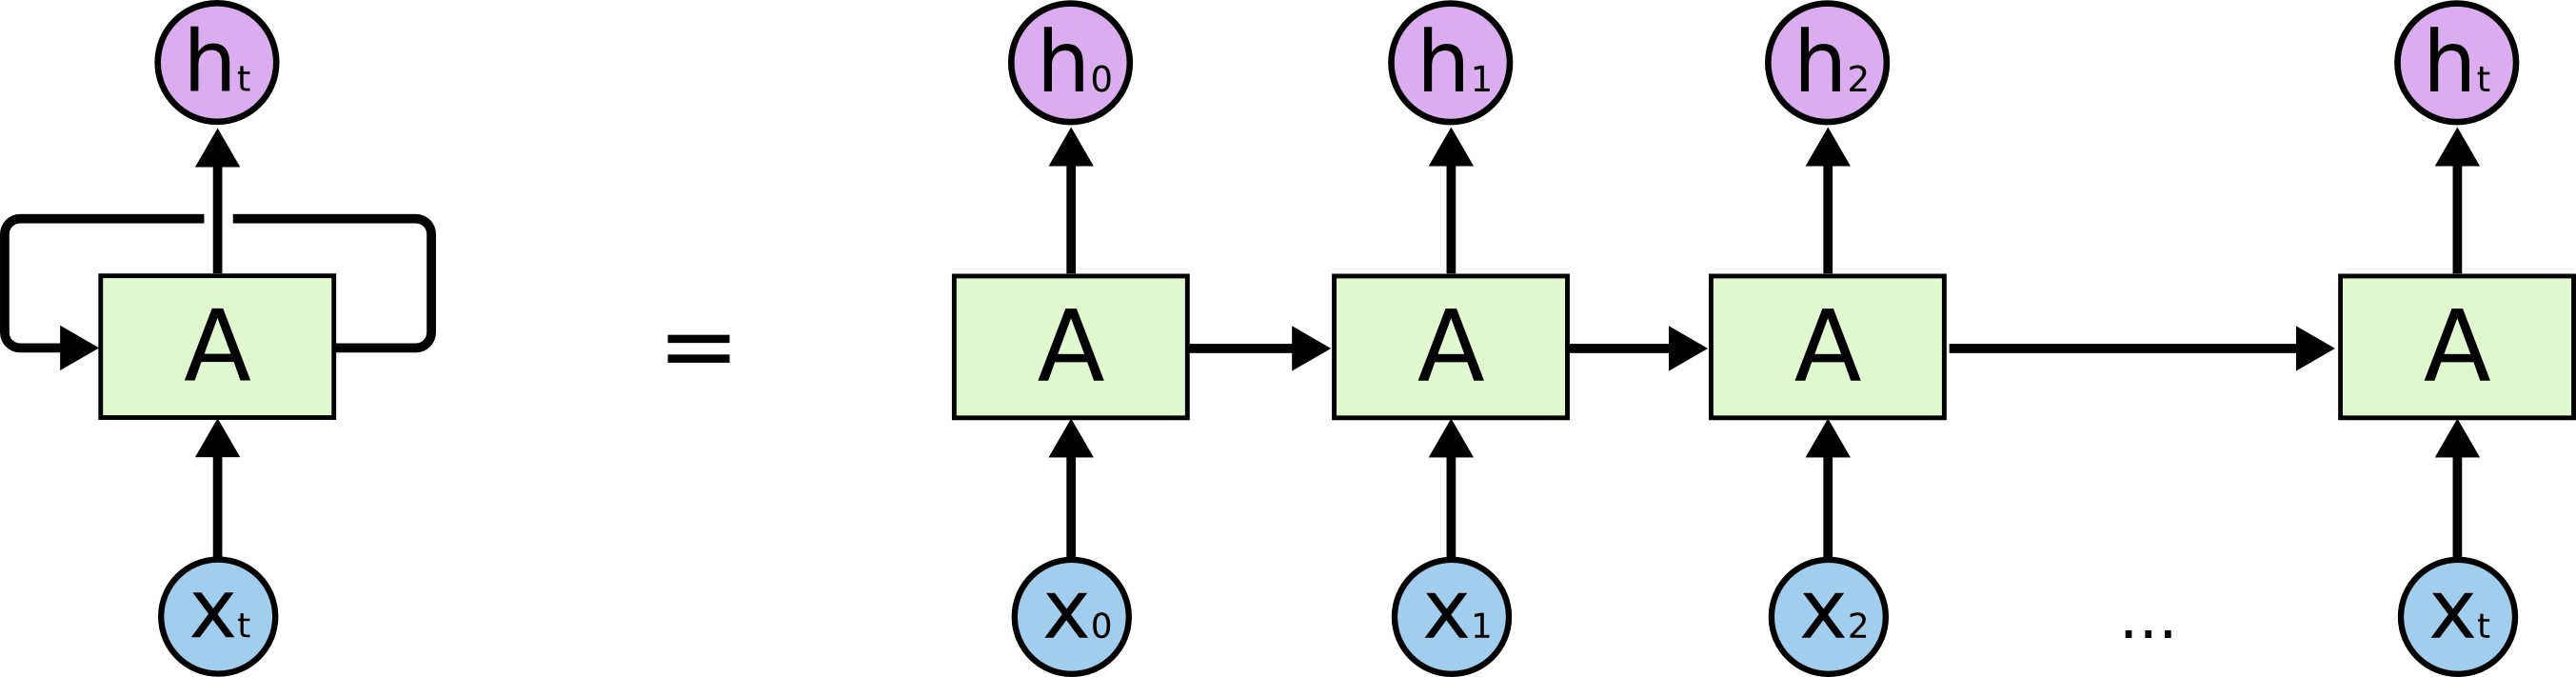
\includegraphics[width=1.0\linewidth]{png/rnn_unrolled}
  \caption{Traditional RNN architechture. Source: https://colah.github.io/posts/2015-08-Understanding-LSTMs/} 
  \label{model_lstm_gru} 
\end{figure}
\subsection{Short Term Memory (LSTM)}
	Long short-term memory (LSTM)~\cite{hochreiter1997long} is a special kind of RNN created for learning long-term dependencies. LSTM units have 3 gates managing the contents of the memory. These gates are simple logistic functions of weighted sums, where the weights might be learnt by backpropagation. It means that, even though it seems a bit complicated, the LSTM perfectly fits into the neural network and its training process. With combining a forget gate in LSTM units, LSTM is capable to determine what it needs to remember and forget, so LSTM can work very well with dependent data , especially with time series data ~\cite{gers2002applying}, ~\cite{guo2016robust}, ~\cite{fu2016using}. The architecture of LSTM units is illustrated in Fig. \ref{model_lstm_gru}, and its mathematical model is briefly described as follows:
	 The input gate (\ref{eq_lstm_1}) and the forget gate (\ref{eq_lstm_2}) manage the cell state (\ref{eq_lstm_4}), which is the long-term memory. The output gate (\ref{eq_lstm_3}) produces the output vector or hidden state (\ref{eq_lstm_5}), which is the memory focused for use. This memory system enables the network to remember for a long time, which was badly missing from vanilla recurrent neural networks. 
	
\begin{align} 
i_t = sigmoid(W_ix_t + U_ih_{t-1}+b_i) \label{eq_lstm_1} \\
f_t = sigmoid(W_fx_t + U_fh_{t-1}+b_f) \label{eq_lstm_2} \\
o_t = sigmoid(W_ox_t + U_oh_{t-1}+b_o) \label{eq_lstm_3} \\
c_t = f_t \odot c_{t-1} + i_t \odot tanh(W_cx_t + U_ch_{t-1} + b_c) \label{eq_lstm_4} \\
h_t = o_t \odot tanh(c_t) \label{eq_lstm_5}
\end{align}

\begin{figure}[!ht] 
   \centering
   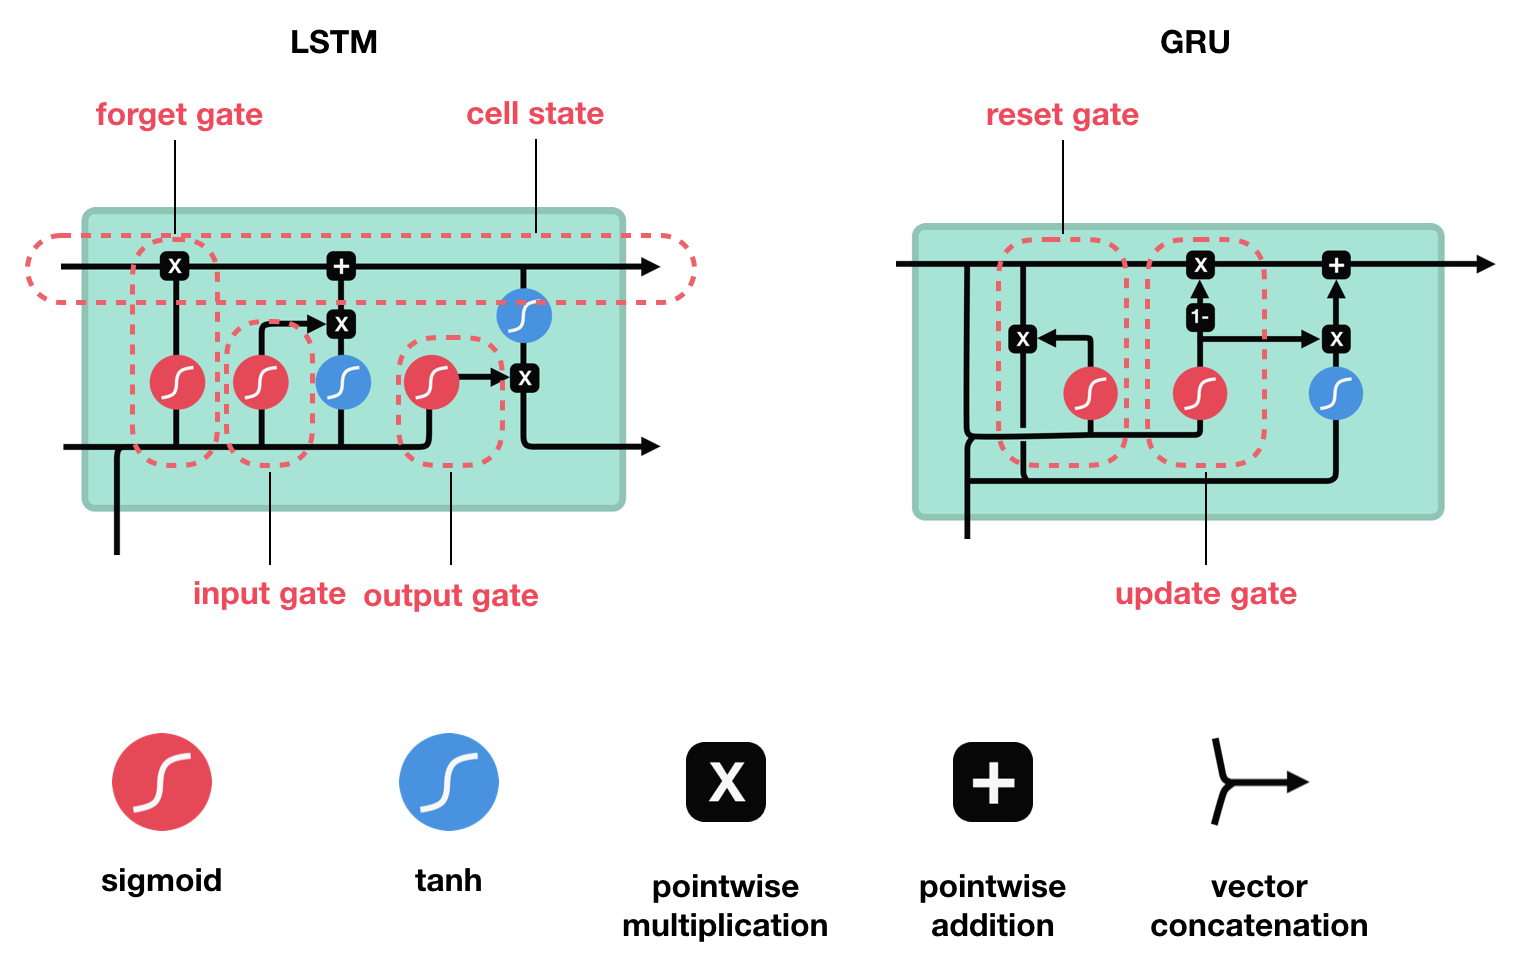
\includegraphics[width=1.0\linewidth]{png/lstm_gru}
  \caption{LSTM and GRU architechture. Source: https://towardsdatascience.com/illustrated-guide-to-lstms-and-gru-s-a-step-by-step-explanation-44e9eb85bf21} 
  \label{model_lstm_gru} 
\end{figure}

\subsection{Gated Recurrent Units (GRU)}

	Gated recurrent unit (GRU)~\cite{chung2014empirical} is essentially a simplified LSTM. Different form LSTM, GRU uses two gated called update gate and reset gate. Basically, these gates are two vectors managing what information should be passed to the output. In GRU, its gates can be trained to keep information from long ago, without washing it through time or remove information which is irrelevant to the prediction. It has the exact same role as LSTM in the network. The main difference is in the number of gates and weights — GRU is somewhat simpler. Like LSTM, GRU is also a widely chosen solution for time series forecasting such as in~\cite{langkvist2014review} and~\cite{bone2000recurrent} The srtucture of GRU units is presented in Fig. \ref{model_lstm_gru} following the mathematical model as below:
	
	The update gate~\ref{eq_gru_1} controls the information flow from the previous activation, and the addition of new information as well~\ref{eq_gru_3}, while the reset gate~\ref{eq_gru_2} is inserted into the candidate activation. Overall, it is pretty similar to LSTM. From these differences alone, it is hard to tell, which one is the better choice for a given problem. 
	
\begin{align} 
z_t = sigmoid(W_zx_t + U_zh_{t−1} + b_z) \label{eq_gru_1} \\
r_t = sigmoid(W_rx_t + U_rh_{t−1} + b_r) \label{eq_gru_2} \\
h_t = z_t\odot h_{t-1} + (1 - z_t)\odot tanh(W_hx_t + U_h(r_th_{t-1}) + b_h) \label{eq_gru_3} \\
\end{align}
\section{Fundamental knowledge}
\label{fun_know}
\subsection{Artificial Neural Network (ANN)}
\label{ann_know}
\subsubsection{Activation functions}
\label{ann_act_func}
	Activation functions also known as transfer functions are used to map input nodes to output nodes in certain fashion. Activation functions are extremely important for an ANN to learn and figure out features and characteristics of data which need a non-linear transformation to become outputs. There are the four most popular functions used in Deep Learning, their names are Sigmoid, Hyperbolic Tangent (Tanh), Rectified Linear Units (ReLU), Leaky ReLU and Exponential Linear Unit (ELU).
	\paragraph{\textbf{Sigmoid function}}: takes a number as input and returns a value in $	[ \,0,1] \,$. (Fig. ****)
	$$f(x) = \frac{1}{1+e^x}$$
	\paragraph{\textbf{Hyperbolic Tangent (Tanh) function:}} $f(x) = \frac{2}{1+e^{-2x}} = 2\sigma(2x)-1$ is also like Sigmoid function but better, the range of the output from Tanh funtion is in $	[ \,-1,1] \,$. (Fig ***)
	$$f(x) = \frac{2}{1+e^{-2x}} = 2\sigma(2x)-1$$
	\paragraph{\textbf{Rectified Linear Unit (ReLU) function:}} is a function having threshold at $0$ value (Fig. ***). It helps accelerate the training process in ANN, so it is used in almost all the complicated deep learning models such as RNNs and CNNs.
	$$f(x) = max(0, x)$$
	\paragraph{\textbf{Leaky ReLU function:}} is like ReLU function, but instead of setting thresholf value at $0$, Leaky ReLU extends the domain to $\alpha x$. (Fig. ****)
	\[
    f(x)= 
\begin{cases}
    x,& \text{if } x > 1\\
    \alpha x, & \text{otherwise}
\end{cases}
\]
	\paragraph{\textbf{Exponential Linear Unit (ELU) function:}} This function was first proposed several years ago. In many experiments, it is proved that it can lead to a faster convergence and better result of deep learning models.
	\[
    f(x)= 
\begin{cases}
    x,& \text{if } x > 1\\
    \alpha (e^x-1), & \text{otherwise}
\end{cases}
\]
\subsubsection{Loss functions}
\label{ann_loss_func}
Neural Networks are trained by backpropagation algorithm, which updates the weights parameters of ANN according to a loss value. The loss value is calculated by a loss function, so loss functions are totally vital when an ANN model is built for learning information from data. These functions will essentially measure how poorly a model is performing by comparing what the model is predicting with the actual value it is supposed to output. Therefore, choosing a loss function that is appropriate for penalizing model effectively is one of the most important tasks while working with data. There are a number of loss functions for deep learning models, and each of them have its own pros and cons. The common loss functions that are widely used in time-series forecasting will be presented as below:
\begin{itemize}
\item  \textbf{Mean Absolute Error (MAE)}: 
$$MAE = \frac{\sum|e_t|}{N}$$
\item  \textbf{Sum Square Error (SSE)}: $$SSE = \sum(e_t^2)$$
\item  \textbf{Mean Square Error (MSE)}: $$MSE = \frac{\sum(e_t^2)}{N}$$
\item  \textbf{Root Mean Square Error (RMSE)}: $$RMSE = \sqrt{MSE}$$
\item  \textbf{Mean Absolute Percentage Error (MAPE)}: $$MAPE = \frac{1}{N}\sum|\frac{e_t}{y_t}|$$
Where $N$ is the number of data points, $y_t$ is the actual output value, $d_t$ is the output value predicted by models, $e_t = d_t - y_t$ is the error value of the data point $t$.
\end{itemize}
	 
\subsubsection{Backpropagation - the ANN Training Algorithm}
\label{ann_backprop_alg}

\begin{algorithm}[!t]
	\caption{Backpropagation algorithm applied for FFNN with 1 hidden layer}
	\label{algorithm_backprop}
	\SetAlgoLined
	Initialize randomly weights' value $w_p$\\ 
	\Repeat{Until convergence or the number of iterations is enough}{
	\textbf{Calculate output value(s) according to weights and input}  \\
	
		\For{$j= 1$ to $h$}
		{
			$H_{j} = \phi(\sum_i^n {x_i*w_{ij}^{[1]} + b_{ij}^{[1]}})$ \\ 
			
		}
		$\widehat {{y_j}} = \phi(\sum_i^h{H_i * w_j^{[2]} + b_j^{[2]}})$\\
		
		\textbf{Calculate Loss value by loss function} \\ 
		
		$L(w) = loss(\widehat {{y_j}},{y_j})  $ \\
		
		 \textbf{Backpropagating Loss to weights}\\
		
		$ \bigtriangleup(w_{ij}^2) = \frac{\partial (L(w))}{\partial (w_{ij}^2)}$ \\
		$ \bigtriangleup(w_{ij}^1) = \frac{\partial (L(w))}{\partial (w_{ij}^1)}$ \\
		
		\textbf{Update weights' value} \\ 
		
		$w_{ij}^2 = w_{ij}^2 - \eta * \bigtriangleup(w_{ij}^2)$ \\
		$w_{ij}^1 = w_{ij}^1 - \eta * \bigtriangleup(w_{ij}^1)$
	}
		
\end{algorithm}

Backpropagation algorithm is undoubtedly the most fundamental buiding block in an ANN. It It was first introduced in 1960s and almost 30 years later (1989) popularized by Rumelhart, Hinton and Williams in~\cite{rumelhart1988learning}. The algorithm is used to effectively train a neural network through a method called chain rule. In simple terms, after each forward pass through a network (propagation phase), backpropagation performs a backward pass while adjusting the model’s parameters (weights and biases) (weights updating phase).

\paragraph{\textbf{forward propagation phase}}
\begin{enumerate}
\item The input values will be fed into ANN through input layer, going forward to hidden layers, and finally to output layer, creating predicted output values. While propagation process, each layer uses its own activation function (sec. \ref{ann_act_func})
\item Error values are calculated by the loss function and propagated back to previous layers.
\end{enumerate}
\paragraph{\textbf{weights updating phase}}

\begin{enumerate}
\item Calculating gradients of loss function in weights and biases following the chain rule.
\item Updating weights and biases is done according to gradients' values 
\end{enumerate}

These two phases are repeated in each iteration during training. The algorithm will be stopped when the error from loss function reach a acceptable value or when the training iteration is large enough. The algorithm's pseudo code is presented in short in Algorithm \ref{algorithm_backprop}.

\subsection{Swarm Optimization Algorithms}
\label{swarm_opt}
\subsubsection{Idea and motivation}
\label{opt_idea}
\subsubsection{Particle Swarm Optimization (PSO)}
\label{pso_standard}
\subsubsection{Sea Lion Optimization Algorithm (SLnO)}
\label{slno_standard}

\begin{algorithm}[!t]
\caption{Sea Lion Optimization (SLnO)}
\label{algorithm_slno}
\SetAlgoLined
 Initialize the Sea Lion population $X_i (i=1,2,.., n)$ randomly. \\
 Calculate fitness of each solution (sea lion). \\
 $X_*\gets$ the best solution \\
\For {$Iter=0 \to Iter_{max}$}{
	Calculate the value of $C$ \\
	\For {SeaLion in population}{\
		Calculate $SP_{leader}$ using Eq. \ref{snlo_eq3}  \\
		\uIf{$SP_{leader} < 0.25$}{
			\uIf {$|C| < 1$}{\
				Update the location of the current search agent using Eq. \ref{slno_eq1}
				}
			\Else {
				Choose a random search agent $SL_{rand}$ \\
				Update the locatiion of current search agent by Eq. \ref{slno_eq8} \\
			}
		}	
		\Else{
			Update the location of the current search agent by Eq. \ref{slno_eq6}
		}
	Evaluate population: fix if any solutions go beyond the boundary \\
 	Recompute the fitness of all solutions \\
 	Check and update $X_*$ if a better solution is found. \\
	}
	
}
 \textbf{Results:}  $X_*, f(X_*)$
\end{algorithm} 

	Sea lions are considered as one of the most intelligent animals in wildlife which live on both lands and the oceans. They usually live in a large swarm with thousands of members, and this large swarm may contains many subgroups with their own hierarchy as well. In each subgroup, there is a dominant sea lion playing a role as the leader of the subgroup. All activities of subgroups are decided following the leader ship of that sea lion.
	
%	The most important characteristics of sea lions is that they have senses helping them to recognize and analyze immediately the movement of their prey such as fish even in the dark underwater environments. Like many predators, sea lions have their eyes point forward so that they can easily focus on the prey, but what makes their eyes different is that they can open pupils so widely to let much of light go through their eyes which helps them to see more clearly in underwater environment. Moreover, sea lions have their super-sensitive whiskers to locate exactly where the fish are. This can be done when the fish swim around, they leave waves or wakes behind them, and according to the intensity as well as the direction of waves, by using whiskers sea lions are able to detect and follow them.
	
	The intelligence of sea lions can be seen through the way they organize their groups and hunt the prey. Hunting as a group allow sea lions to have more opportunities of obtaining more food especially when the amount of fish is quite large. Usually, sea lions capture their prey together by circling the prey in a narrow ball, and the size of this "ball" continues to be decrease until the prey is totally wiped out. The main phases of hunting behaviors of sea lions can be illustrated as 3 steps as follows:
	
\begin{itemize}
\item Tracking and chasing the prey using their senses.
\item Calling other members to gather and implement encircling strategy around the prey.
\item Attack towards the prey which is captured in the circle.
\end{itemize}

	Those behaviors is the inspiration for the Sea Lion Optimization (SLnO) which was first introduced in ~\cite{masadeh2019sea}. The algorithm mimics the amazing social behaviors and interesting hunting activities of sea lions. The formulas of the phases \textit{Detecting and tracking phase}, \textit{Vocalization phase} and \textit{Attacking phase} illustrate perfectly encircling mechanisms which is utilized by sea lions. We summarize and discuss briefly each phase in the algorithm as below, meanwhile the pseudo-code of SLnO is provided in details in \textbf{Algorithm \ref{algorithm_slno}}.

\begin{enumerate}
\item \textbf{Detecting and tracking phase}

	Sea lions can identify the location of the prey and gather other members that will join the subgroup to organize the net following the encircling mechanism. This sea lion plays an important role as a leader for this hunting behavior and other members' position will be updated following the position of the prey. In SLnO algorithm, the prey is considered as the current best solution or the solution closest to the optimal solution. This behaviors is presented mathematically using Eq. (\ref{slno_eq1}) and Eq. (\ref{snlo_eq2}) as follows:
\begin{align}
Dist = |2B.P(t) - SL(t)| \label{slno_eq1} \\
SL(t+1) = P(t) - Dist.C  \label{snlo_eq2}
\end{align}
	
	Where $Dist$ indicates the distance between the prey and the current sea lion; $P(t)$ and $SL(t)$ represent the position vectors of best solution and the sea lion in iteration $t$ respectively; $B$ is random vector in the range $[0, 1]$ which is multiplied by 2 to increase the search space, helping the search agent find optimal or near optimal position. $SL(t+1)$ is the new position of search agent after updating and $C$ is linearly decreased from 2 to 0 over the course of iterations, indicating the encircling mechanism of sea lion group when they move towards the prey and surround them.

\item \textbf{Vocalization phase}
	
	When a sea lion recognize a group of their prey (such as fish), it will call other sea lions in their group for gathering and creating a net to capture the prey. That sea lion is considered as the leader and it will lead the group of sea lions moving towards and decide the behaviors of the group. These behaviors are modeled mathematically as shown in Eq. (\ref{snlo_eq3}), (\ref{snlo_eq4}) and (\ref{snlo_eq5}):
	
\begin{align} 
SP_{leader} = |(V_1(1+V_2)/V_2| \label{snlo_eq3} \\
V_1 = \sin(\theta) \label{snlo_eq4} \\
V_2 = \sin(\phi) \label{snlo_eq5}
\end{align}


 Where $SP_{leader}$ is the value that illustrates the decision of the leader followed by other sea lions in the group; $\theta$ and $\phi$ are the angles of its voice's reflection and refraction in the water, respectively.
 
\item \textbf{Attacking phase (Exploitation phase)}
 
 The hunting activities of sea lions are led by the leader. In SLnO algorithm, the target prey is considered the current best candidate solution. In order to mathematically mimic the hunting behaviors of sea lions, two phases are introduced as follows:
 	
\begin{itemize}
\item \textit{Dwindling encircling technique:}
	This behavior depends on the value of $C$ in Eq. \ref{snlo_eq2}. $C$ is linearly decreased from 2 to 0 over the course of iterations, so this allows the search space around the current best position to shrink and force other search agents to updated in this search space as well. Therefore, a new updated position of a sea lion can be located anywhere in the search space between its current position and the location of the present best agent.

\item \textit{Circling updating position}: Sea lions chase bait ball of fishes and hunt them starting from edges. Eq. \ref{slno_eq6} is proposed in this regard:
\begin{equation} \label{slno_eq6}
SL(t+1) = |P(t) - SL(t)|.\cos(2 \pi m) + P(t)
\end{equation}	
\end{itemize}
	Where $|P(t) - SL(t)|$ illustrates the distance between the best optimal solution (the prey) and the current search agent in t-th iteration, $||$ means the absolute value and $m$ is a random number in the range $[-1, 1]$.
	
\item \textbf{Searching for prey (Exploration phase)}
	In exploration phase, the search agents update their positions based on a randomly selected sea lion. The condition that allows exploitation phase to happen is when the value of $C$ becomes greater than 1, and the process of finding a new agent is presented by Eq. (\ref{slno_eq7}) and (\ref{slno_eq8}) as below:
\begin{align}
Dist = |2B.SL_{rnd}(t) - SL(t)| \label{slno_eq7} \\
SL(t+1) = SL_{rnd}(t) - Dist.C \label{slno_eq8}
\end{align}   

	Where $SL_{rnd}(t)$ is a random sea lion that is selected randomly from current population.

\end{enumerate}	

\chapter{Improved Sea Lion Optimization (ISLO) algorithm and Proposed Model for Auto-Scaling (ISLO-CFNN)}
\section{Improved Sea Lion Optimization (ISLO)}
\label{improved_ISLO}
	Sea Lion Optimization (SLnO) is one of the newest swarm-based optimization algorithm. In experiments in SLnO origin paper \cite{masadeh2019sea}, SLnO is proved that it outperformed several well-known bio-inspired model such as Generic Algorithm (GA), Particle Swarm Optimization (PSO) and Whale Optimization Algorithm (WOA). However, like many other algorithms, SLnO also faces the problem of local minimum, slow convergence and diversity degradation of population. In SLnO's exploitation phase, the updating operation \ref{slno_eq2} only takes the distance between the current agent and the best solution into account, which makes updated position always oriented to one direction, leading to poverty of exploitation ability. Also, in exploration phase, although the participation of two agents that already exist in population in the updating operation \ref{slno_eq8} helps the new-born solution inherits current decent features of population, new solution has no way to reach another position outside of existing positions. This results in a dramatic decrease in the diversity of population, and significantly influences the ability of escaping local minimum of SLnO algorithm. All things considered, we decided to enhance those 2 operators by taking individual information into account for exploitation phase, and using a technique called opposition-based operation for exploration phase. These two improvements form a new version of SLnO called Improved Sea Lion Optimization (ISLO) algorithm. The pseudo code of the algorithm is presented in Algorithm \ref{algorithm_islo}, and  our improvements would be discussed in detail in \ref{imprv_exploit} and \ref{imprv_explore} as below.  
\begin{algorithm}[!t]
\caption{Improved Sea Lion Optimization (ISLO)}
\label{algorithm_islo}
\SetAlgoLined
 Initialize the Sea Lion population $X_i (i=1,2,.., n)$ randomly. \\
 Calculate fitness of each solution (sea lion). \\
 $X_*\gets$ the best solution \\
\For {$Iter=0 \to Iter_{max}$}{
	Calculate the value of $C$ \\
	\For {SeaLion in population}{\
		Calculate $SP_{leader}$ using Eq. \ref{snlo_eq3}  \\
		\uIf{$SP_{leader} < 0.25$}{
			\uIf {$|C| < 1$}{\
				Calculate $Dist_1$ and $Dist_2$ using Eq. \ref{islo_eq1} and \ref{islo_eq2}
				Update the location of the current search agent using Eq. \ref{islo_eq3}
				}
			\Else {
				Choose a random search agent $SL1_{rand}$ and $SL2_{rand}$ \\
				Update the location of current search agent by Eq. \ref{islo_eq4} \\
			}
		}	
		\Else{
			Update the location of the current search agent by Eq. \ref{slno_eq6}
		}
	Evaluate population: fix if any solutions go beyond the boundary \\
 	Recompute the fitness of all solutions \\
 	Check and update $X_*$ if a better solution is found. \\
	}

}
 \textbf{Results:}  $X_*, f(X_*)$
\end{algorithm}   
\subsection{Exploitation phase improvement}
\label{imprv_exploit}
	As mentioned above, SLnO have its own drawbacks in its exploitation phase. In order to enhance the performance of the operation \ref{slno_eq2}, not only distance between the current agent and the best agent, but also the influences of an individual experiment in history is considered in new improved operation. This idea stems from the updating mechanism of PSO \cite{eberhart1995particle} where the velocity of a particular particle is influenced by both the best individual and best personal information. ***************.
	
	Following that idea, we apply the information sent from best individual experiment in the same way as best agent position. The direction of position movement affected by two factors is presented in Fig. ***, and along with it,  the formulas of new updating mechanism for exploitation phase is as follows:
\begin{equation}\label{islo_eq1}
Dist_1 = |2B.P(t) - SL(t)| 
\end{equation}
\begin{equation}\label{islo_eq2}
Dist_2 = |2B.P_i(t) - SL(t)| 
\end{equation}
\begin{equation}\label{islo_eq3}
SL(t+1) = r_1(P(t) - Dist_1.C) + r_2(P_i(t) - Dist_2.C)
\end{equation}
where $P_i(t)$ is the personal best position of agent $i$ up to time $t$, and $r1, r2$ are random numbers in range $[\, 0,1 ] \,$.

	In new operation \ref{islo_eq3}, the new-updated position of an individual is the result of adding two vectors, one is the vector presenting the direction of that individual towards the best agent, and another is the direction towards its own experiences in history. The influences of both two factors are determined by two random numbers $r_1$ and $r_2$. $r_1$ and $r_2$ play an extremely important role in the updating mechanism,  because  they create random characteristics for the operation, helping ISLO avoiding local minimum and taking advantages of the two factors. Without the appearance of $r_1$ and $r_2$, the updated position is always affected exactly half by best agent and half by its experience, which may lead to degradation of the diversity of population. 

\subsection{Exploration phase improvement}
	
	In origin SLnO algorithm, new-born agents that are created in exploration phase cause a poor exploration search ability because of inheriting features of existing solutions. In order to tackle this problem, exploration phase is required the operation to have the ability of creating a decent new-born solution. New updated position need to satisfy two characteristics: carrying random features for ensuring a strong capability of exploration phase, and landing in a position decent enough (close enough to the best agent position) for updating positions in the next generation. From that motivation, a method called Opposition-based Learning (OBL) \cite{tizhoosh2005opposition}, which is successfully applied for enhancing bio-inspired optimization algorithms such as GA \cite{tizhoosh2005opposition}, PSO \cite{wang2007opposition} \cite{tang2009enhanced} in solving several optimization problems including finding parameter for deep learning models \cite{rashid2010improved} \cite{nguyen2019efficient} is utilized as a base model for our improvement in exploration operation of SLnO. 
	
	
	The idea of OBL is applied in the operation in the way of finding a new random optimal solution, but still retain a part of features from existing solutions. This is done by calculating the opposed position to the current position of an living agent in population. For ensuring random characteristics of new found position, a random agent from population, and a random agent in the search space will be chosen for participating in this operation. Fig. *** illustrates corresponding position of new solution given two positions of each factor, and the process as well as mathematical formulas are given as follows:
\begin{enumerate}
\item Select a random solution $SL1_{rand}$ in the search space.
\item Select a random existing solution $SL2_{rand}$ in the population.
\item Create a new solution $SL_{rand}$ by calculating the opposed position to $SL1_{rand}$ through $SL2_{rand}$.
\begin{equation} \label{islo_eq4}
SL_{rand} = 2*SL2_{rand} - SL1_{rand}
\end{equation}
\end{enumerate}

\section{Proposed model for auto-scaling problem in Cloud Computing}
\label{proposed_model}
	
	In chapter \ref{ch:background}, we generally discussed about Cloud Computing and the problem of auto-scaling with the existing methods for solving this. In general, it is relatively necessary to build cloud computing servers with the capacity of automatically expanding and  shrinking the resources allocated. Although there are a number of solutions proposed for tackling this issue, they all have their own drawbacks.
	
	The FFNN model, which is widely used for solving many real-world issues, is too simple to capture the characteristics of time-series data because after feed-forwarding through hidden layers, the origin information of the input neural could be forgotten. On the other hand, RNN-based models such as LSTM or GRU have to face the problem of extremely complex structures that potentially lead to over-fitting, or the huge number of hyper-parameters which are needed to tuned.
	
	The CFNN can take the advantages of its structure and diminish the problem raising when the model structures are too simple (FFNN) or too complex (LSTM, GRU) because of the connection added between the input layer and output layer. However, the gradient descent (GD) algorithm which is used for optimizing CFNN still have its own drawback of being stuck in local minimum and slow convergence speed. 
	
	All thing considered, we proposed a new model ISLO-CFNN to improve the weak points of origin CFNN model by replacing GD algorithm by above proposed ISLO algorithm in optimizing the parameters of the network while training process. Also, in order to evaluate the performance of our proposed model, we would build both our model and existing models for the purposes of evaluation and comparison.
	
	
	
	Fig. \ref{fig_model_phases} illustrates the skeleton of forecasting system designed. There are four main phases, each of them is indispensable in our model. The phases are Collecting data, Data pre-processing, Building and Training model and Deploy prediction model. Firstly, historical records about resources used are collected and saved in lines in a log file. These information is extracted and pre-processed before being used for training the prediction model that is designed. In the final stage, the trained model is applied for data in current time, and it will predict the amount of resources needed. Specifically, in Building and Training model stage, CFNN model is built with fixed nodes in all layers, and it will be optimized by ISLO algorithm, which is discussed in detail in Section \ref{improved_ISLO}. We will discuss about each phase as below.
	
\begin{figure}[!ht] 
   \centering
   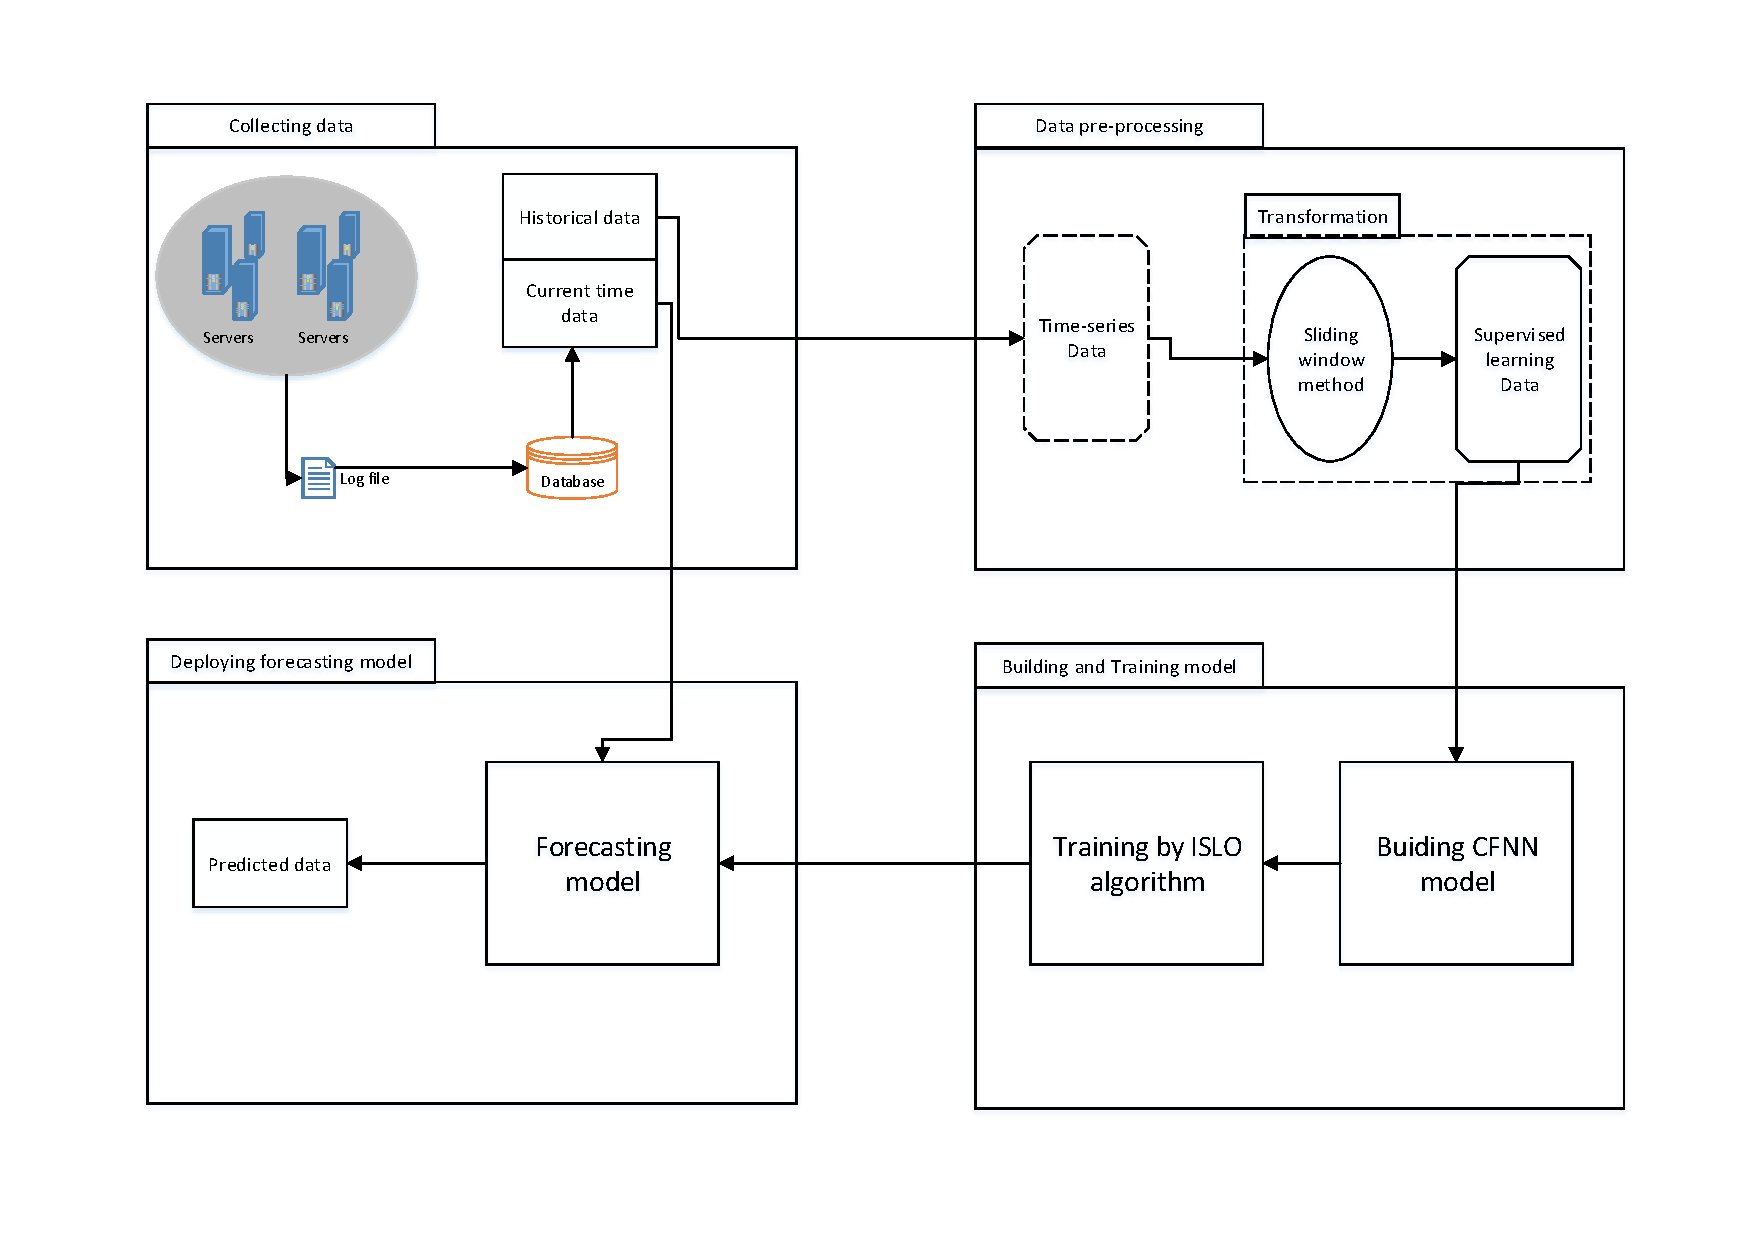
\includegraphics[width=1.0\linewidth]{/pdf/model/model_phases}
  \caption{Proposed model design} 
  \label{fig_model_phases} 
\end{figure}
	
\subsection{Collecting data}
\label{collect_data}
	
	Before building any forecasting systems, the very first and the most important task that must be done is collecting data. Therefore, we collect data recording the resource usage of Google (Google Cluster Trace data) and Internet Traffic data collected from a private internet service provider (ISP) in Europe and the United Kingdom (these datasets  will be discuss in detail in Chapter \ref{experiments}). The data collected contains two main parts: the data from history that we use for training, and current time data that we use for predicting resource usage in the future.  
	

\subsection{Data pre-processing}
\label{data-pre}

\begin{table}[!t]
\caption{Time-series data and Supervised learning data comparison}
\label{tbl_data_cmp}
\centering
\begin{tabular}{|p{6cm}|p{6cm}|}
 \hline
 Time-series data & Supervised Learning data  \\ 
 \hline
 1. Time 1, value 1 & 1. Input 1, output 1  \\ 
 2. Time 2, value 2 & 2. Input 2, output 2  \\ 
 3. Time 3, value 3 & 3. Input 3, output 3  \\ 
 \hline
\end{tabular}
\end{table}
	
	This phase play a role as a pre-processor transforming the raw data into the kind of data that can be used in neural networks. In order to learn, models need both training data and testing data. We create the data for models through several steps as follows:

\begin{itemize}
\item  Evaluate and choose carefully which columns of data are needed for the forecasting model.
\item  The parts of data chosen are then normalized in the range $[ \, 0, 1 ] \,$.
\item Transform time-series data into supervised learning data using \textit{Sliding window} technique.
\item Divide processed data into two sets: training set and testing set.
\end{itemize}

	The step $3th$ of the pre-processing phase is necessary because time-series data is the data recorded through time, and there is no term of features and output data. Therefore, we need to transform this data into supervised learning data, that contains input features, and output. Table \ref{tbl_data_cmp} depicts the difference between time-series data and normal data used in supervised learning.


	In order to create data for supervised learning, we use the method called \textit{Sliding window}. This method takes the data of $k$ values before the time $t$ as the features and output data is the value at the time $t$. For example, when $k=3$, the results of data transformation is shown as in Table \ref{tbl_sliding_window}.
	
\begin{table}[!t]
\caption{Example of data transformation using Sliding window method}
\label{tbl_sliding_window}
\centering
\begin{tabular}{|p{4cm}|p{2cm}|p{2cm}|p{2cm}|p{2cm}|}
 \hline
 \multicolumn{1}{|c|}{Time-series data} & \multicolumn{4}{c|}{Transformed data} \\ 
 \hline
 \multicolumn{1}{|c}{} & \multicolumn{3}{|c}{Input} & \multicolumn{1}{|c|}{Output} \\
 \hline
  Time $(t=4)$, Value 4 & Value 1 & Value 2 & Value 3 & Value 4 \\
  Time $(t=5)$, Value 5 & Value 2 & Value 3 & Value 4 & Value 5 \\
  Time $(t=6)$, Value 6 & Value 3 & Value 4 & Value 5 & Value 6 \\
  Time $(t=7)$, Value 7 & Value 4 & Value 5 & Value 6 & Value 7 \\
 ... & ... & ... & ...  & ... \\
 \hline
\end{tabular}
\end{table}	
	 
\subsection{Building and Training model}
\label{main_model}

	In this phase, pre-processed data is used for training our proposed model called ISLO-CFNN, which is CFNN trained under the optimization of ISLO algorithm. ISLO algorithm is applied to train a CFNN model with one hidden layer. There is two key aspects needed to be taken into consideration: firstly, the formation of an agent in ISLO and the selection of fitness function.
	
	Firstly, each agent in the population in ISLO are presented as one solution for CFNN model, which means a search agent is a one-dimensional vector created by concatenating weights and biases of CFNN. Therefore, the features of a search agent contains three elements: a set of weights connecting the input layer with hidden layer, a set of weights connecting the hidden layer with output layer and also, a set of weights connecting the input layer with output layer. Therefore,  the length of a solution can be calculated by Eq. \ref{eq_length_solution}.
	
\begin{equation} \label{eq_length_solution}
	Solution\_length = (1+i)*h + (1+h)*o + (1+i)*o
\end{equation}
Where $i, h, o$ is the number of input, hidden and output neurons,  respectively (in time-series prediction, the number of output neurons is one).
	
	Secondly, the fitness value of each agent in ISLO is considered as the loss value of the CFNN model with the parameter set from the agent and input data. We utilize the loss function Mean Square Error (MSE) to calculate the difference between the actual and predicted output values by generated agent for all samples in the training set. 
	
	The workflow of ISLO applied in this work for training CFNN can be presented by the following steps:
	
\begin{enumerate}
\item Initialization: pre-define the number of search agents in ISLO, which are randomly generated in the range [0, 1]. Each search agent presents a solution for CFNN model.
\item Calculate fitness value for each search agent: The quality of a solution is measured by the loss value of CFNN output. After being decoded into weights and biases vectors, a solution will be applied to form a CFNN model. Data samples in training set is then feed-forwarded through the network, generating predicted output values. Finally, the fitness value is calculated as the difference between predicted and actual output values through the MSE loss function.
\item Update positions of all search agents following formulas of ISLO algorithm.
\item Steps 2 and 3 are repeated until the difference is close enough, or the maximum number of iterations is reached.
\end{enumerate}
	     
	
	
	

\subsection{Deploy prediction model}
\label{deploy}  
	  
\chapter{Experiments}
\chapter{Conclusions}

\appendix
% appendices come here

\bibliographystyle{plain}
\bibliography{references}
%\addcontentsline{toc}{chapter}{Bibliography}
%\bibliographystyle{alpha}
%\bibliography{bibliography/bibliography}

\end{document}